\newpage
\section{Auswertung}
\label{sec:Auswertung}
\subsection{Statische Messung}
\begin{figure}[h!]
	\label{fig:overview1}
	\centering
	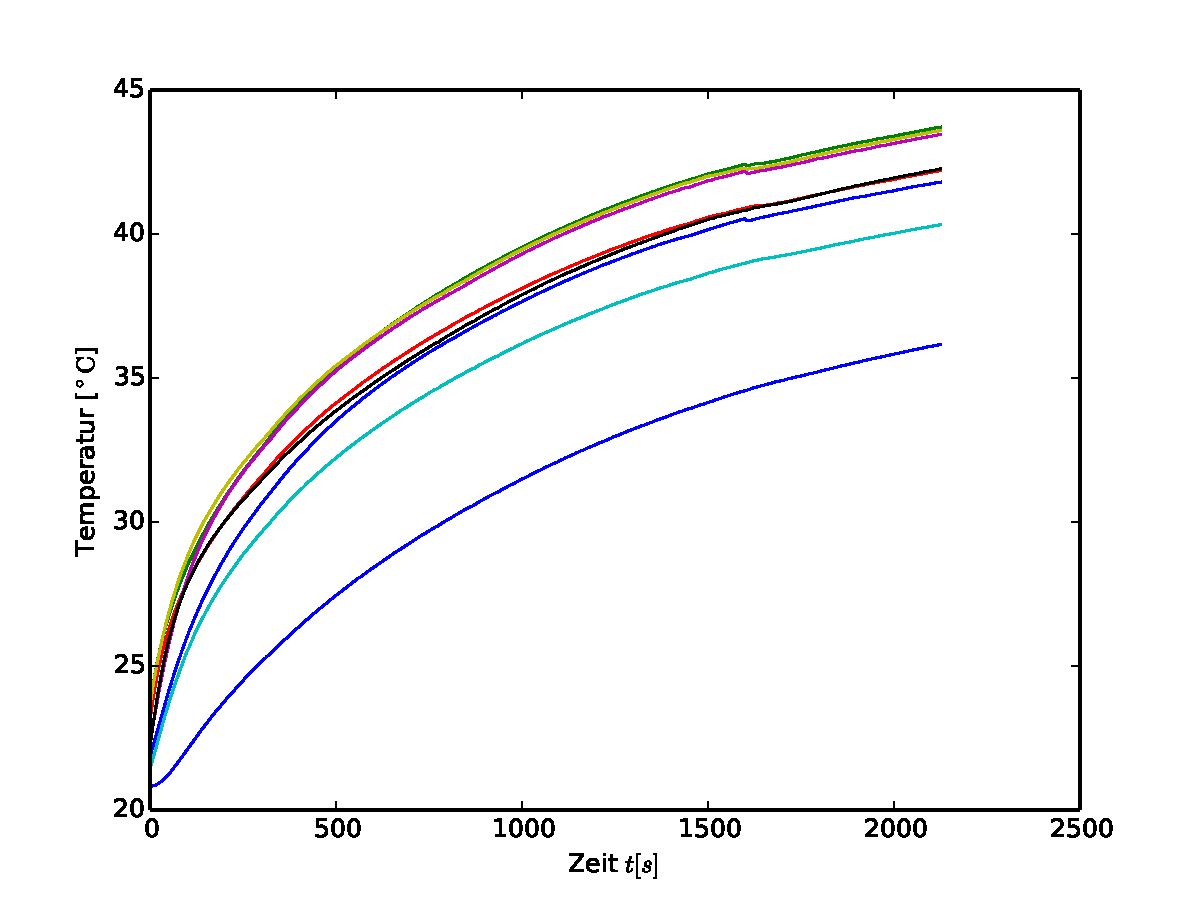
\includegraphics[width=0.7\textwidth]{Bilder/M1_Overview.pdf}
	\caption{Alle gemessenen Temperaturen}
\end{figure}
Alle Temperaturverläufe werden in Diagramm \ref{fig:overview1} gleichzeitig aufgetragen. Es zeigt, dass der allgmeine Verlauf der Temperatur unabhängig von dem Material und der Entfernung des Messpunktes ist. Die Temperaturkurven zeigen jeweils beschränktes Wachstum.

\begin{figure}[p]
	\label{fig:entftemp}
	\centering
	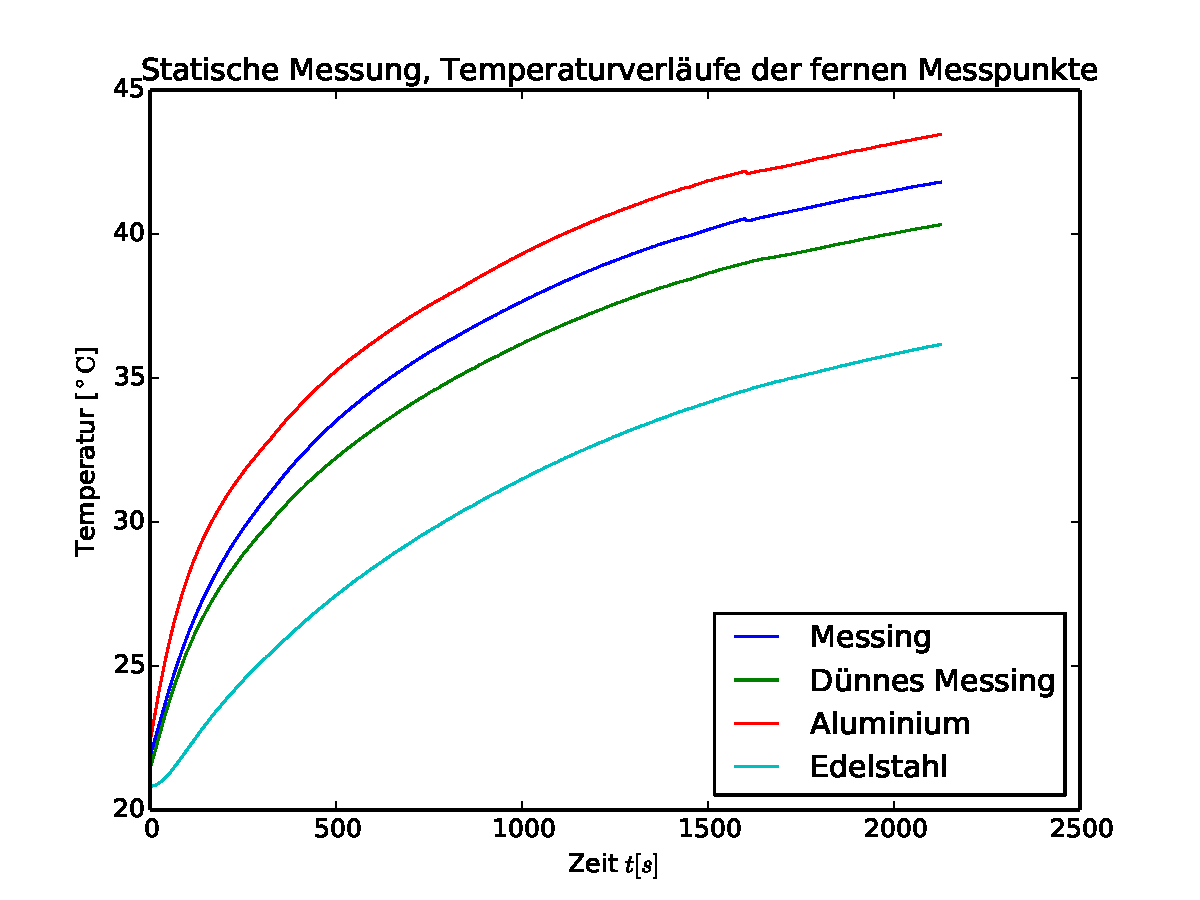
\includegraphics[width=0.8\textwidth]{Bilder/M1_Tempverl.pdf}
	\caption{Verlauf der Temperaturen an den entfernten Messpunkten}
\end{figure}
Im Diagramm \ref{fig:entftemp} wird der Temperaturverlauf bei den entfernten Messpunkten T1, T4, T5, T8 (vgl. \ref{fig:platine}) gezeigt. 
Die Kurve von Aluminium hat zu Beginn des Experiments den stärksten Anstieg und liegt über den Kurven der anderen Metallstäbe. 
Beide Kurven der Messingstäbe haben vergleichbare Steigungen;
die Kurve des größeren Messingstabes liegt dabei über der des kleineren Stabes und hat am Endpunkt der Messung zu dieser eine Temperaturdifferenz von etwa $1 \si{\degreeCelsius}$. 
Die Kurve von Edelstahl ist deutlich von den Kurven der anderen Metallstäbe entfernt und weist die geringste Steigung auf. 
Zum Endpunkt der Messung liegt zwischen den Messpunkten von Aluminium und Edelstahl eine maximale Temperaturdifferenz von etwa $7 \si{\degreeCelsius}$ vor. 

Cirka 700 Sekunden nach Beginn des Erwärmens liegen an den entfernten Messpunkten die Temperaturen nach Tabelle \ref{tab:700} vor. 
\begin{table}[h!]
\centering
\begin{tabular}{cccc}
	\toprule
	{Edelstahl}&{Messing,dünn}&{Messing}&{Aluminium}\\
	\midrule
	29$\si{\degreeCelsius}$& 34$\si{\degreeCelsius}$& 35.4$\si{\degreeCelsius}$& 37$\si{\degreeCelsius}$\\
	\bottomrule
\end{tabular}
\label{tab:700}
\caption{Temperaturen an entfernten Messpunkten bei $t=700\si{\second}$}
\end{table}
Die höchste Temperatur hat der Aluminiumstab, die geringste Temperatur weist Edelstahl auf.

Mit \eqref{waermemenge} kann der Wärmestrom $\frac{\Delta{Q}}{\Delta{t}}$ innerhalb der Stäbe bestimmt werden. 
Hierzu ist in \eqref{waermemenge} $\kappa$ der Litearaturwert der Wärmeleitfähigkeit des betrachteten Metalls und $A$ die Querschnittsfläche (vgl. hierzu \cite{V204}) des jeweiligen Stabes; $\frac{\partial T}{\partial x}$ ist der Temperaturgradient innerhalb des Stabes und wird hier mit $\frac{\Delta T}{\Delta x}$ und $\Delta x$genähert.
Es ergibt sich für die Wärmemenge $\mathup{d}Q$ zu fünf unterschiedlichen Zeiten\\
%\begin{table}
%\centering
%\begin{tabular}{ccccc}
%	\multicolumn{5}{c}{Messing}\\
%	\toprule
%	Nach $500\si{\second}$&Nach $1000\si{\second}$& Nach $1500\si{\second}$&Nach $2000\si{\second}$& Nach $50\si{\second}$\\
%	$-0.3552\si{\watt}$&$-0.36288\si{\watt}$&$-0.37248\si{\watt}$&$-0.3648\si{\watt}$&$-0.49728\si{\watt}$\\
%	\bottomrule
%\end{tabular}
%\end{table}
%\begin{table}[h!]
%\centering
%\begin{tabular}{ccccc}
%	\multicolumn{5}{c}{Messing, dünn}\\
%	\toprule
%	Nach $500\si{\second}$&Nach $1000\si{\second}$& Nach $1500\si{\second}$&Nach $2000\si{\second}$& Nach $50\si{\second}$\\
%	$-0.2128\si{\watt}$&$-0.21504\si{\watt}$&$-0.21728\si{\watt}$&$-0.21056\si{\watt}$&$-0.28672\si{\watt}$\\
%	\bottomrule
%\end{tabular}
%\end{table}
%\begin{table}[h!]
%\centering
%\begin{tabular}{ccccc}
%	\multicolumn{5}{c}{Aluminium}\\
%	\toprule
%	Nach $500\si{\second}$&Nach $1000\si{\second}$& Nach $1500\si{\second}$&Nach $2000\si{\second}$& Nach $50\si{\second}$\\
%
%	$-0.06768\si{\watt}$&$-0.0564\si{\watt}$&$-0.0564\si{\watt}$&$-0.04888\si{\watt}$&$-0.41736\si{\watt}$\\
%	\bottomrule
%\end{tabular}
%\end{table}
%\begin{table}[h!]
%\centering
%\begin{tabular}{ccccc}
%	\multicolumn{5}{c}{Edelstahl}\\
%	\toprule
%	Nach $500\si{\second}$&Nach $1000\si{\second}$& Nach $1500\si{\second}$&Nach $2000\si{\second}$& Nach $50\si{\second}$\\
%	$-0.15384\si{\watt}$&$-0.1536\si{\watt}$&$-0.1524\si{\watt}$&$-0.14688\si{\watt}$&$-0.1116\si{\watt}$\\
%	\bottomrule
%\end{tabular}
%\end{table}
\begin{table}
\centering
\begin{tabular}{cccccc}
\sisetup{table-format=1.4}\\
%\multicolumn{1c}{Probe}{4c}{Zeiten}\\
Stab & $50\:\si\second$ & $500\:\si\second$ & $1000\:\si\second$ & $1500\:\si\second$ & $2000\:\si\second$ \\
\toprule
Messing 1 &$-0.4973\:\si{\watt}$ &$-0.3552\:\si{\watt}$&$-0.3629\:\si{\watt}$&$-0.3725\:\si{\watt}$&$-0.3648\:\si{\watt}$\\
Messing 2 &$-0.2867\:\si{\watt}$& $-0.2128\:\si{\watt}$&$-0.2150\:\si{\watt}$&$-0.2173\:\si{\watt}$&$-0.2106\:\si{\watt}$\\
Aluminium &$-0.4174\:\si{\watt}$&$-0.0677\:\si{\watt}$&$-0.0564\:\si{\watt}$&$-0.0564\:\si{\watt}$&$-0.0489\:\si{\watt}$\\
Edelstahl &$-0.1116\:\si{\watt}$&$-0.1538\:\si{\watt}$&$-0.1536\:\si{\watt}$&$-0.1524\:\si{\watt}$&$-0.1469\:\si{\watt}$\\
\bottomrule
\label{tab:waememengen}
\end{tabular}
\caption{Wärmemengen d$Q$ der Probenstäbe zu fünf unterschiedlichen Zeiten}
\end{table}

\begin{figure}[htp]
	\label{fig:tempverl}
	\centering
	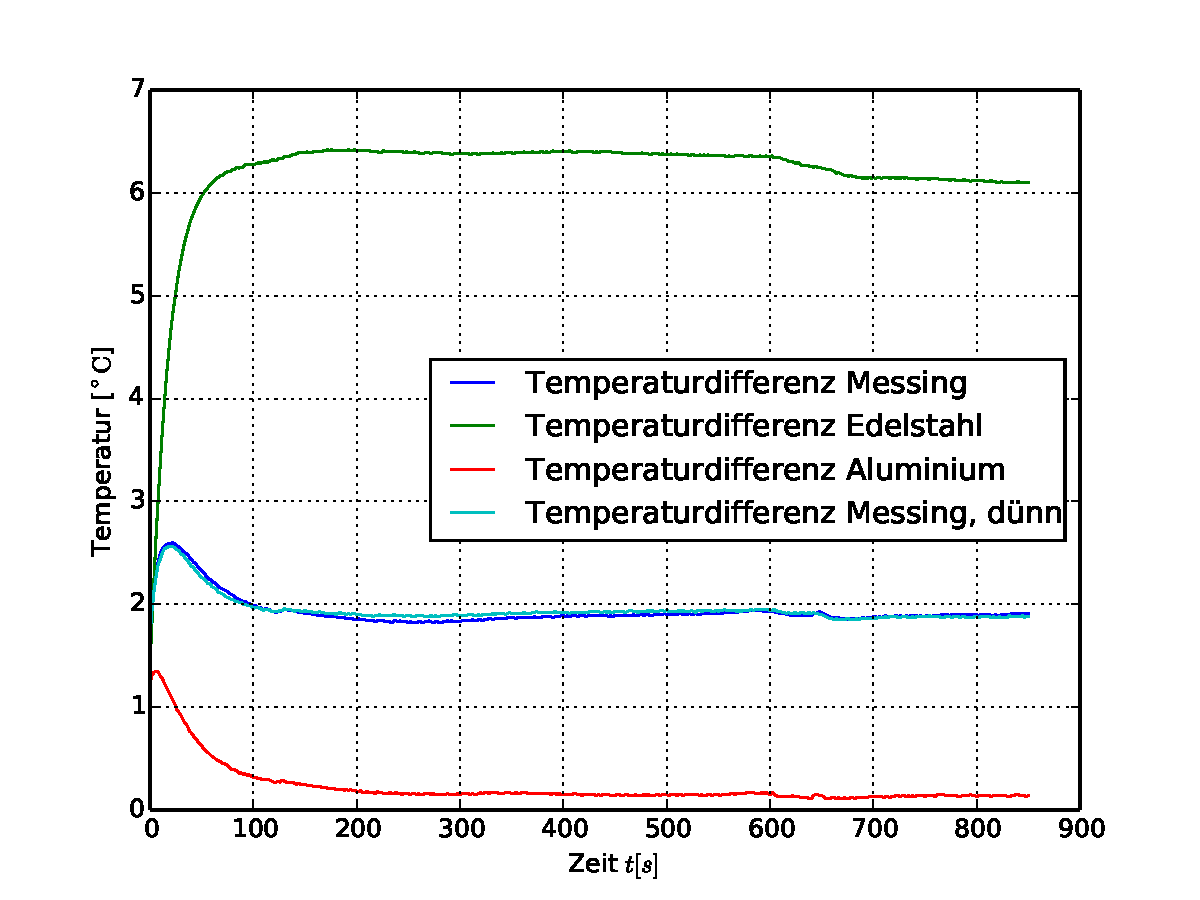
\includegraphics[width=0.8\textwidth]{Bilder/M1_Tempdiff.pdf}
	\caption{Temperaturdifferenz der Messpunkte von Messing und Edelstahl}
\end{figure}

Im Diagramm \ref{fig:tempverl} ist die Temperaturdifferenz innerhalb eines Stabes für den Edelstahl- und für den Messingstab aufgetragen. 
Es wird deutlich, dass die Differenzkurve für Edelstahl näherungsweise ein beschränktes Wachstum beschreibt und kurz nach Beginn der Erwärmung einen Grenzwert erreicht, der bei etwa  $6.25 \si{\degreeCelsius}$ liegt.
Die Differenzkurve des Messingstabes steigt zu Beginn der Messung an und erreicht kurz nach Beginn mit $2.6 \si{\degreeCelsius}$ ihr globales Maximum. 
Nach dem Maximum nimmt die Differenz exponentiell ab und erreicht einen Grenzwert von etwa $2 \si{\degreeCelsius}$.
Der Vergleich der Kurven zeigt, dass der Messingstab gegenüber dem Edelstahlstab den Grenzwert der Temperaturdifferenz schneller erreicht.

\subsection{Dynamische Messung mit 80 Sekunden-Periode}
Die Diagramme \ref{fig:M2Messing} zeigen bei periodischer Anregung einer Temperaturwelle mit einer Periodendauer von 80 Sekunden den Temperaturverlauf an den jeweiligen Enden. 
Zusätzlich zum Verlauf sind sowohl die Extrema, als auch deren Amplitudenfunktion eingezeichnet. 
Analoges Vorgehen mit den Werten für den Aluminiumstab ergeben die Diagramme \ref{fig:M2Alu} und \ref{fig:M2AluNorm}.
Die Messwerte ab dem neunten lokalen Maximum werden von der Auswertung aufgrund offensichtlicher Abweichungen ausgeschlossen.

Normiert man den Temperaturverlauf mit der eingezeichneten Amplitudenfunktionen, so ergeben sich normierte Schwingungen in Diagramm \ref{fig:M2MessingNorm} und \ref{fig:M2AluNorm}. In diesen Diagrammen ist zu erkennen, dass sich für eine gleichmäßige Schwingung jeweils die oberen Amplitudenfunktionen zur Normierung eignen.

\begin{figure}[htp]
\label{fig:M2Messing}
\centering
	\begin{subfigure}{0.9\textwidth}
	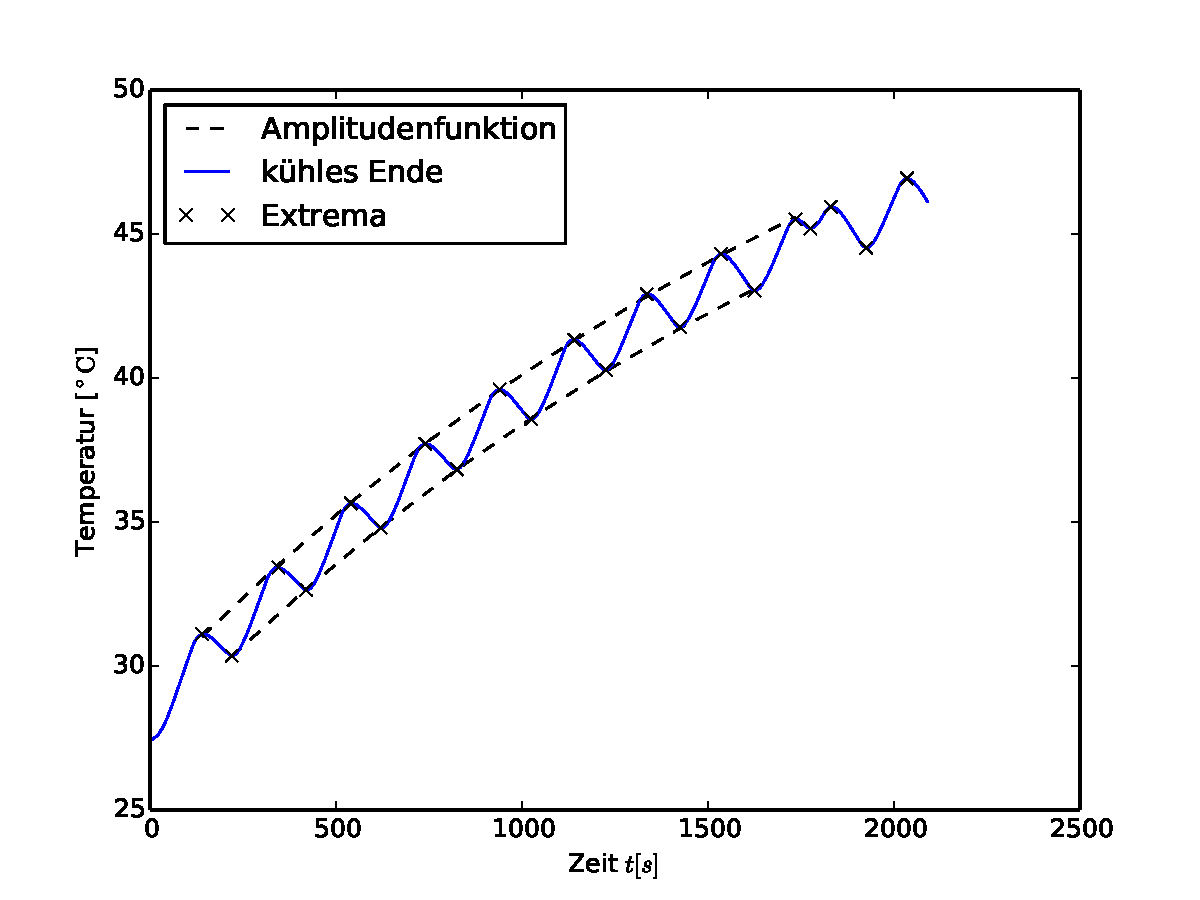
\includegraphics[width=\textwidth]{Bilder/M2_Messing_kuehl.pdf}
	\end{subfigure}
	\begin{subfigure}{0.9\textwidth}
	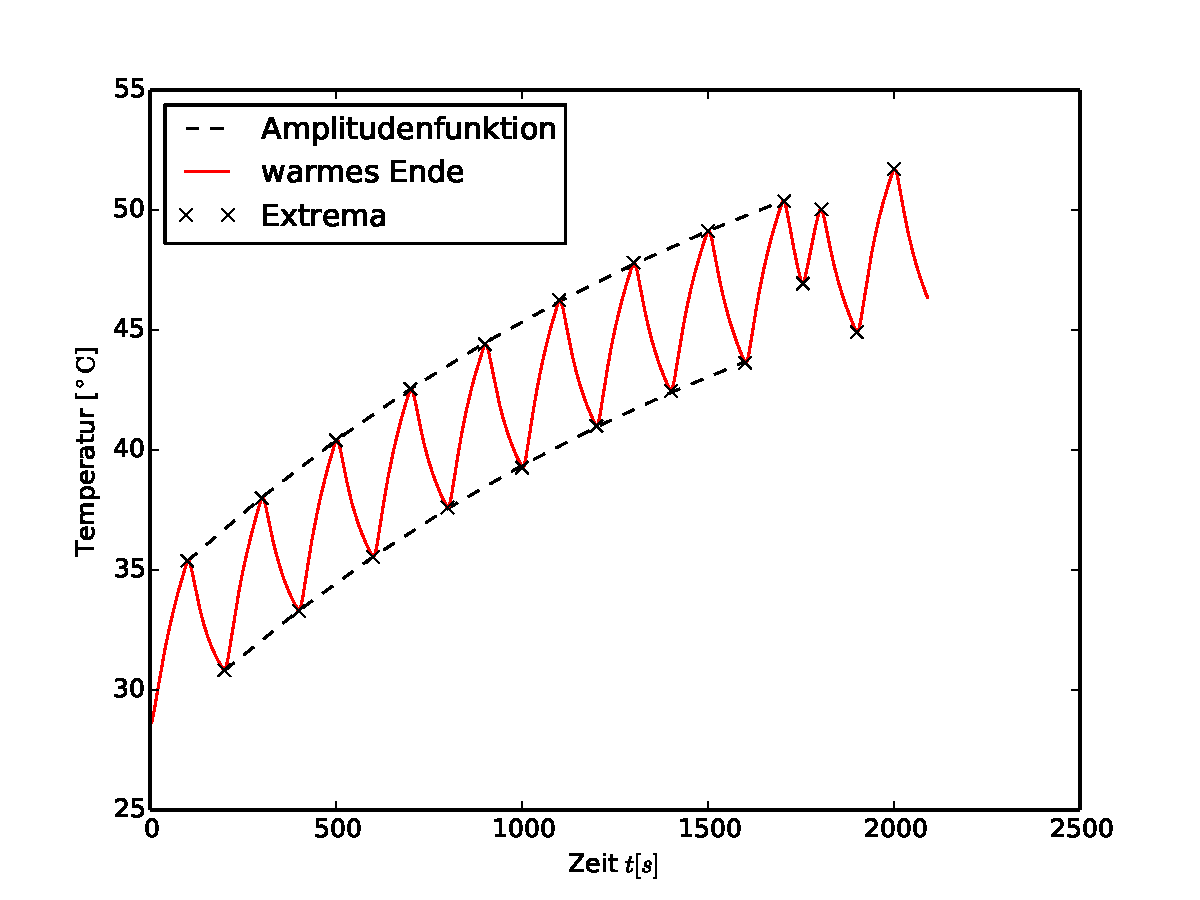
\includegraphics[width=\textwidth]{Bilder/M2_Messing_warm.pdf}
	\end{subfigure}
\caption{Periodische Messung bei Messing mit 80 Sekunden-Periode}
\end{figure}
\begin{figure}[htp]
\label{fig:M2Alu}
\centering
	\begin{subfigure}{0.9\textwidth}
	\centering
	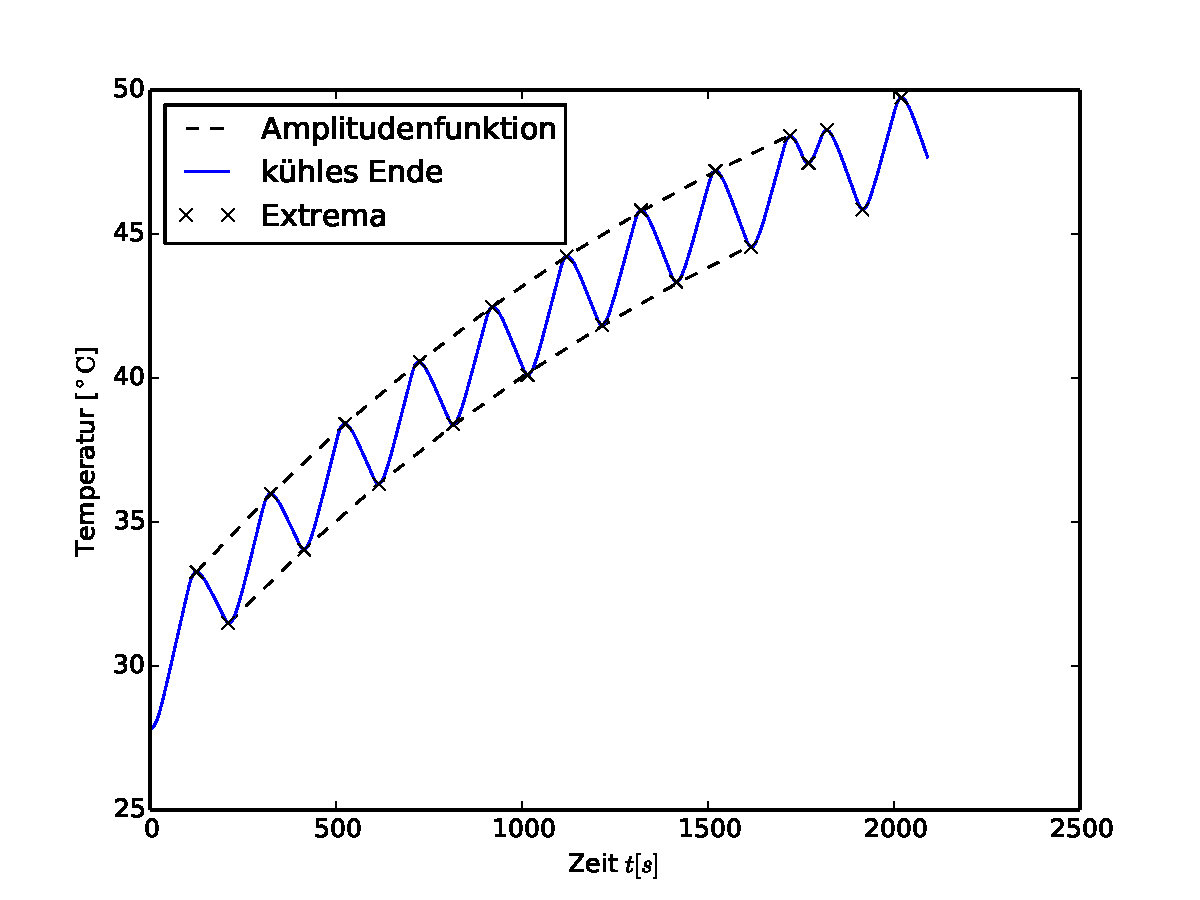
\includegraphics[width=\textwidth]{Bilder/M2_Alu_kuehl.pdf}
	\end{subfigure}
	\begin{subfigure}{0.9\textwidth}
	\centering
	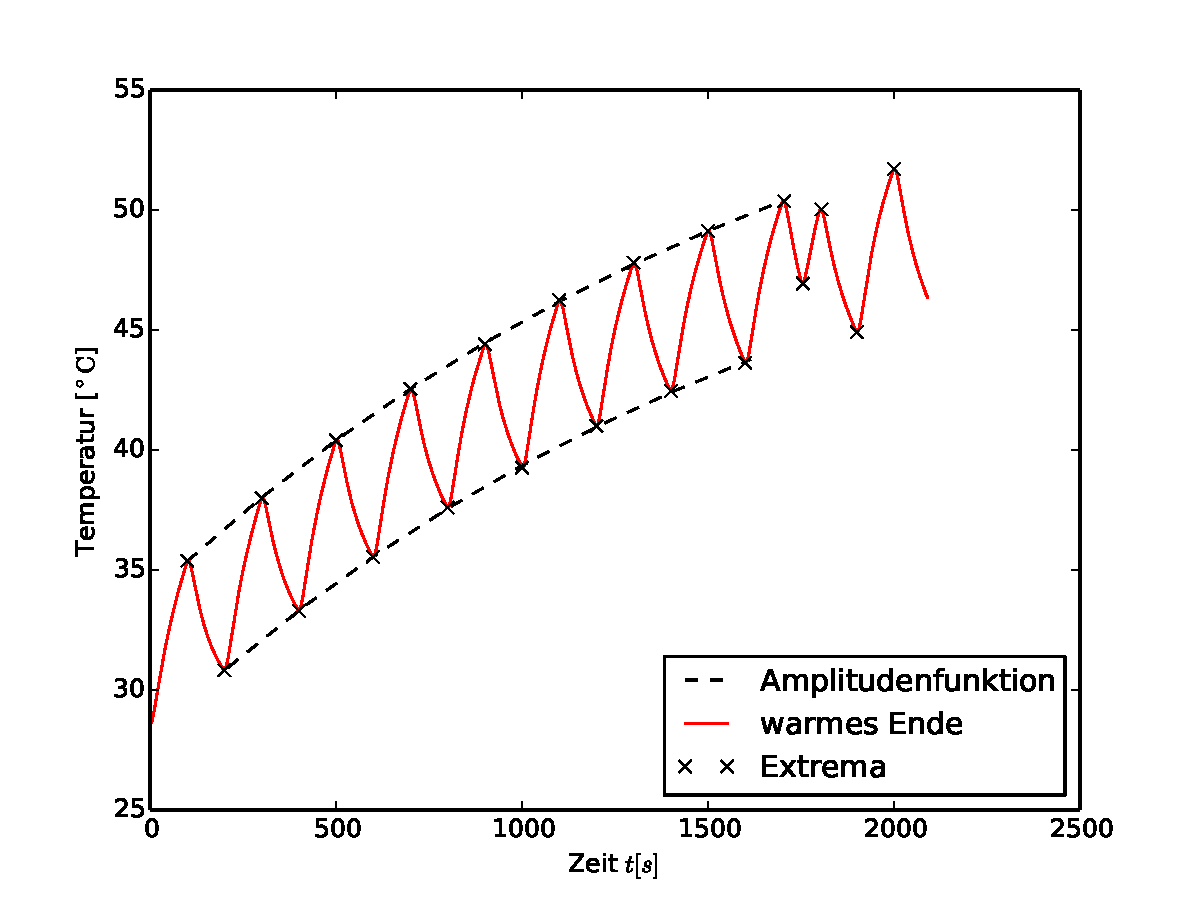
\includegraphics[width=\textwidth]{Bilder/M2_Alu_warm.pdf}
	\end{subfigure}
\caption{Periodische Messung bei Aluminium mit 80 Sekunden-Periode}
\end{figure}
\begin{figure}[htp]
	\label{fig:M2MessingNorm}
	\centering
	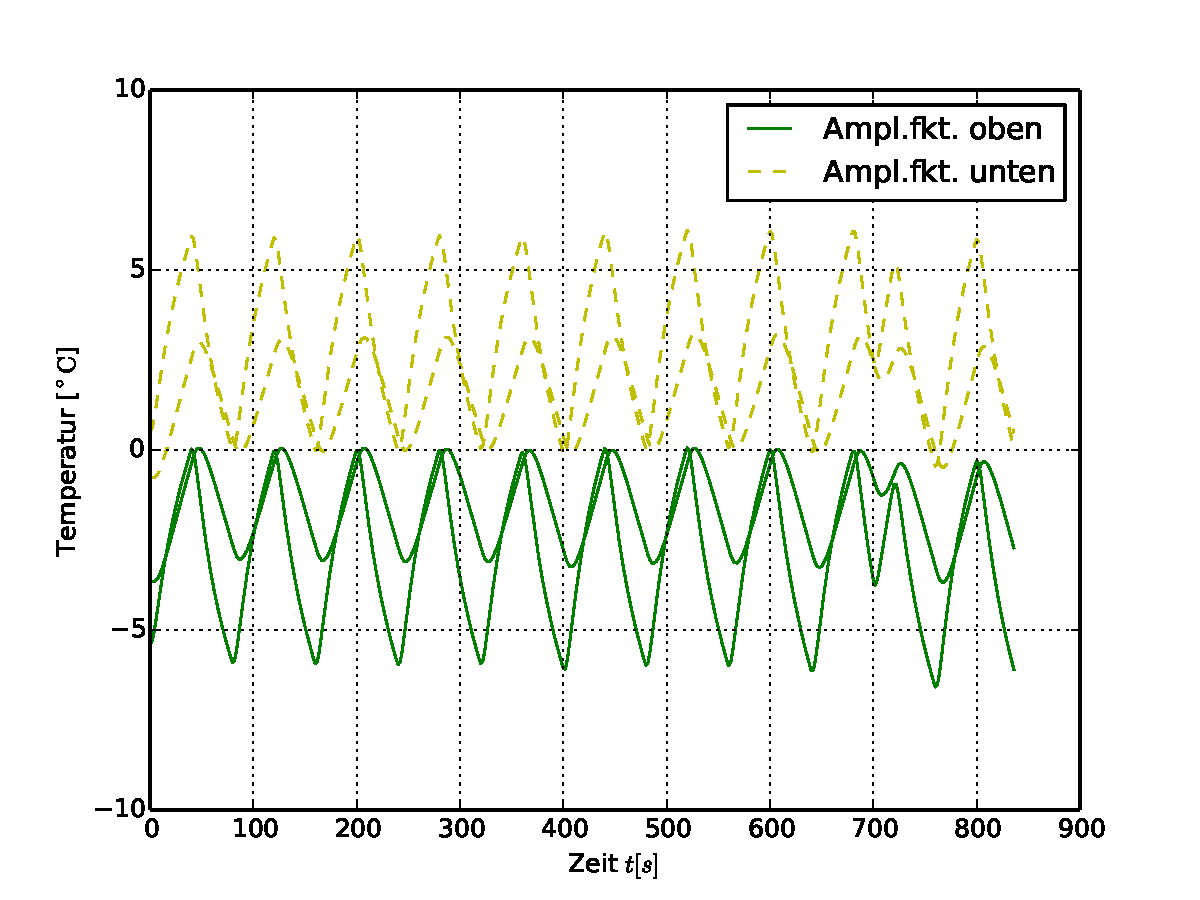
\includegraphics[width=0.8\textwidth]{Bilder/Normierungsauswahl/M2_Alu_norm.pdf}
	\caption{Normierung von Diagramm \ref{fig:M2Alu} auf Grundschwingung}
\end{figure}
\begin{figure}[htp]
	\label{fig:M2AluNorm}
	\centering
	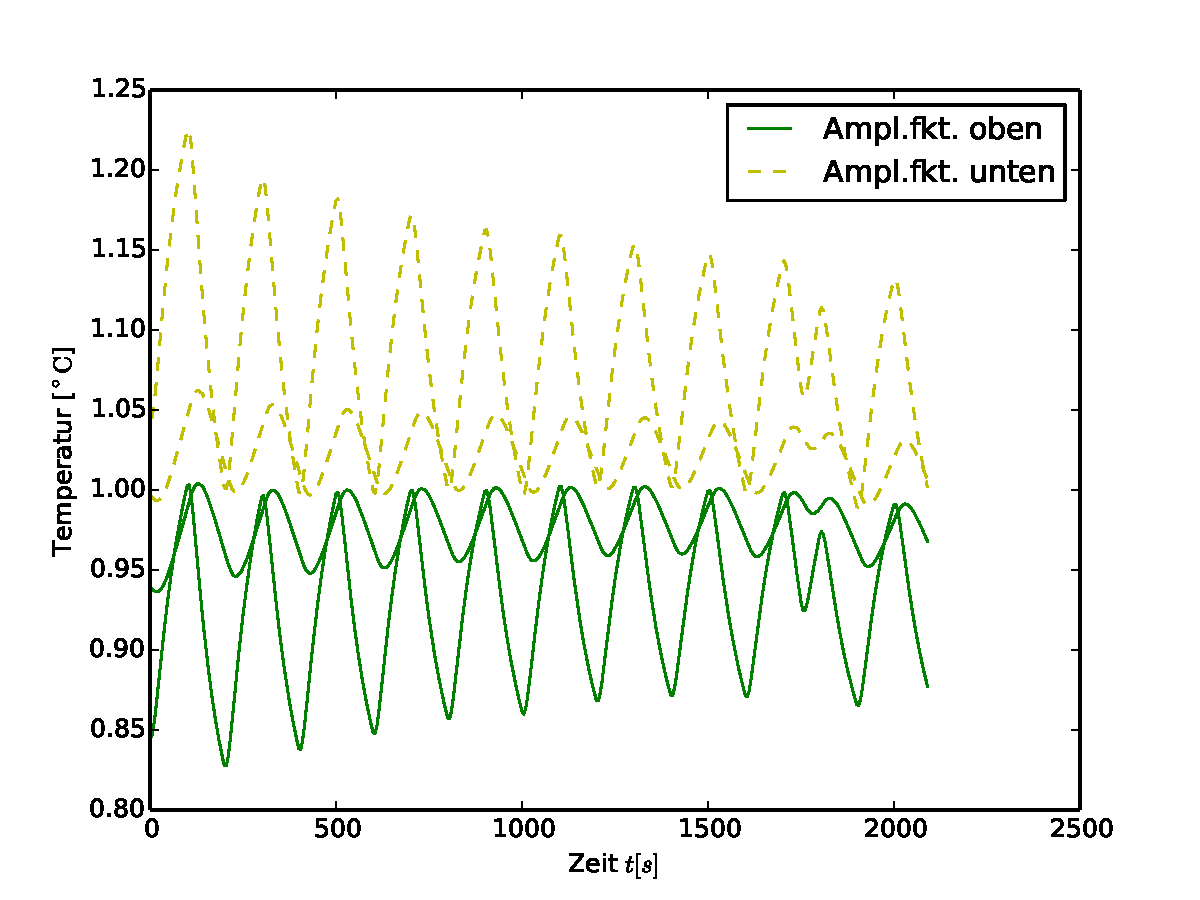
\includegraphics[width=0.8\textwidth]{Bilder/Normierungsauswahl/M2_Messing_norm.pdf}
	\caption{Normierung von Diagramm \ref{fig:M2Messing} auf Grundschwingung}
\end{figure}
\subsection{Dynamische Messung mit 200 Sekunden-Periode}
Die Diagramme \ref{fig:M3Messing} zeigen bei periodischer Anregung einer Temperaturwelle mit einer Periodendauer von 200 Sekunden den Temperaturverlauf an den jeweiligen Enden. 
Zusätzlich zum Verlauf sind die Extrema markiert und erneut deren Amplitudenfunktionen abgebildet.
Analoges Vorgehen mit den Werten für den Aluminiumstab und den Edelstahlstab ergeben die Diagramme \ref{fig:M3Alu}, \ref{fig:M3AluNorm}, \ref{fig:M3Edelstahl} und \ref{fig:M3EdelstahlNorm}.

Normiert man den Temperaturverlauf mit der eingezeichneten Amplitudenfunktionen, so ergeben sich normierte Schwingungen in Diagramm \ref{fig:M3MessingNorm}, \ref{fig:M3AluNorm} und\ref{fig:M3EdelstahlNorm}. Man erkennt anhand dieser Diagramme, dass sich jeweils die oberen Amplitudenfunktionen dazu eignen, den Temperaturverlauf eine gleichmäßige Grundschwingung zu normieren.

\begin{figure}[htp]
\label{fig:M3Messing}
\centering
	\begin{subfigure}{0.9\textwidth}
	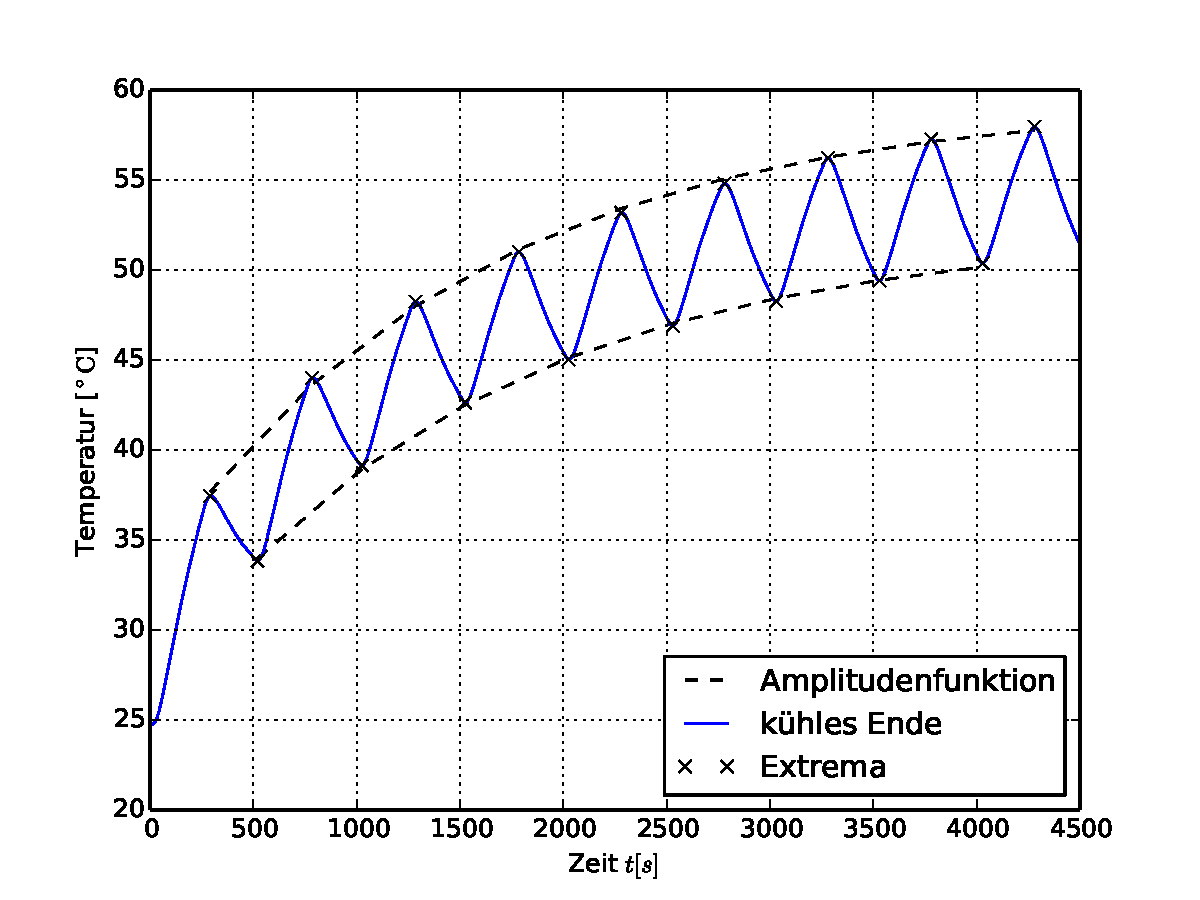
\includegraphics[width=\textwidth]{Bilder/M3_Messing_kuehl.pdf}
	\end{subfigure}
	\begin{subfigure}{0.9\textwidth}
	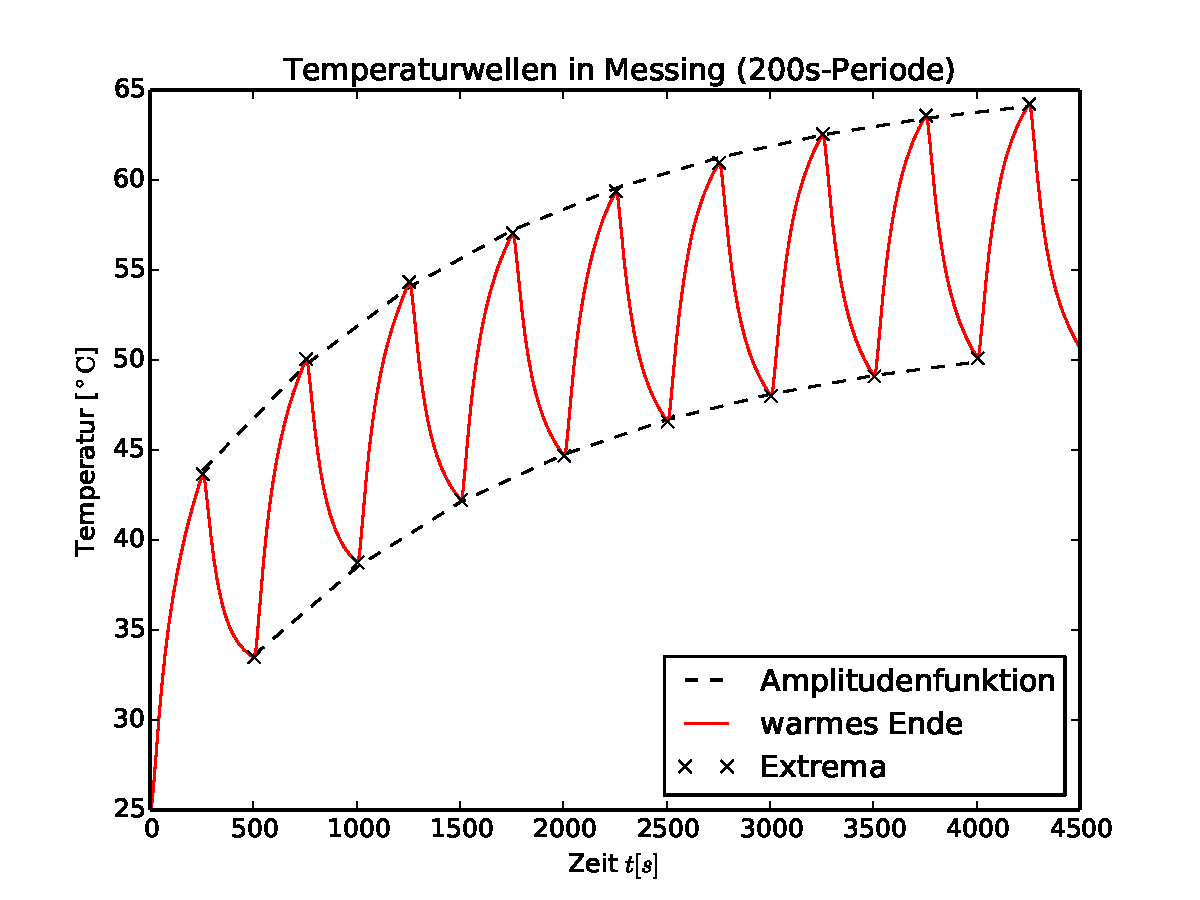
\includegraphics[width=\textwidth]{Bilder/M3_Messing_warm.pdf}
	\end{subfigure}
\caption{Periodische Messung bei Messing mit 200 Sekunden-Periode}
\end{figure}
\begin{figure}[htp]
\label{fig:M3Alu}
\centering
	\begin{subfigure}{0.9\textwidth}
	\centering
	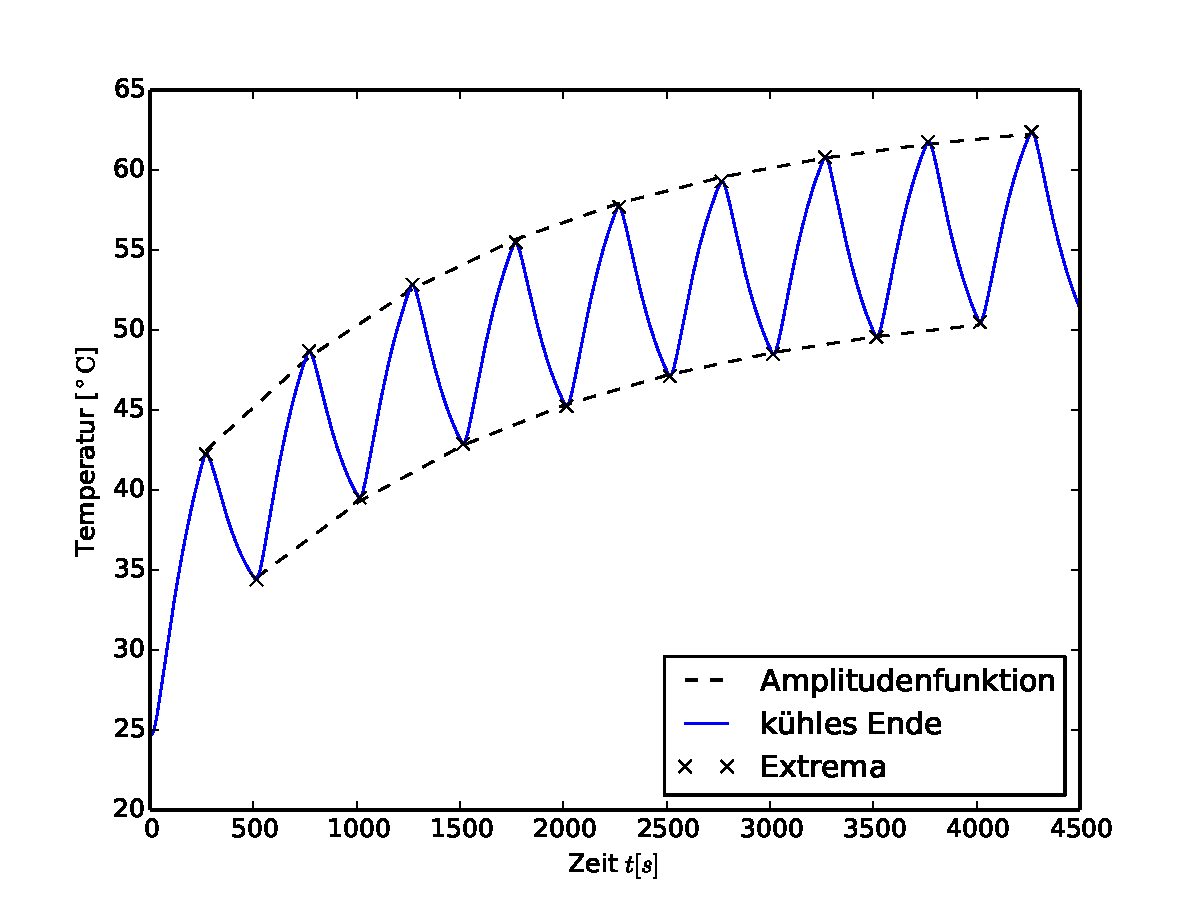
\includegraphics[width=\textwidth]{Bilder/M3_Alu_kuehl.pdf}
	\end{subfigure}
	\begin{subfigure}{0.9\textwidth}
	\centering
	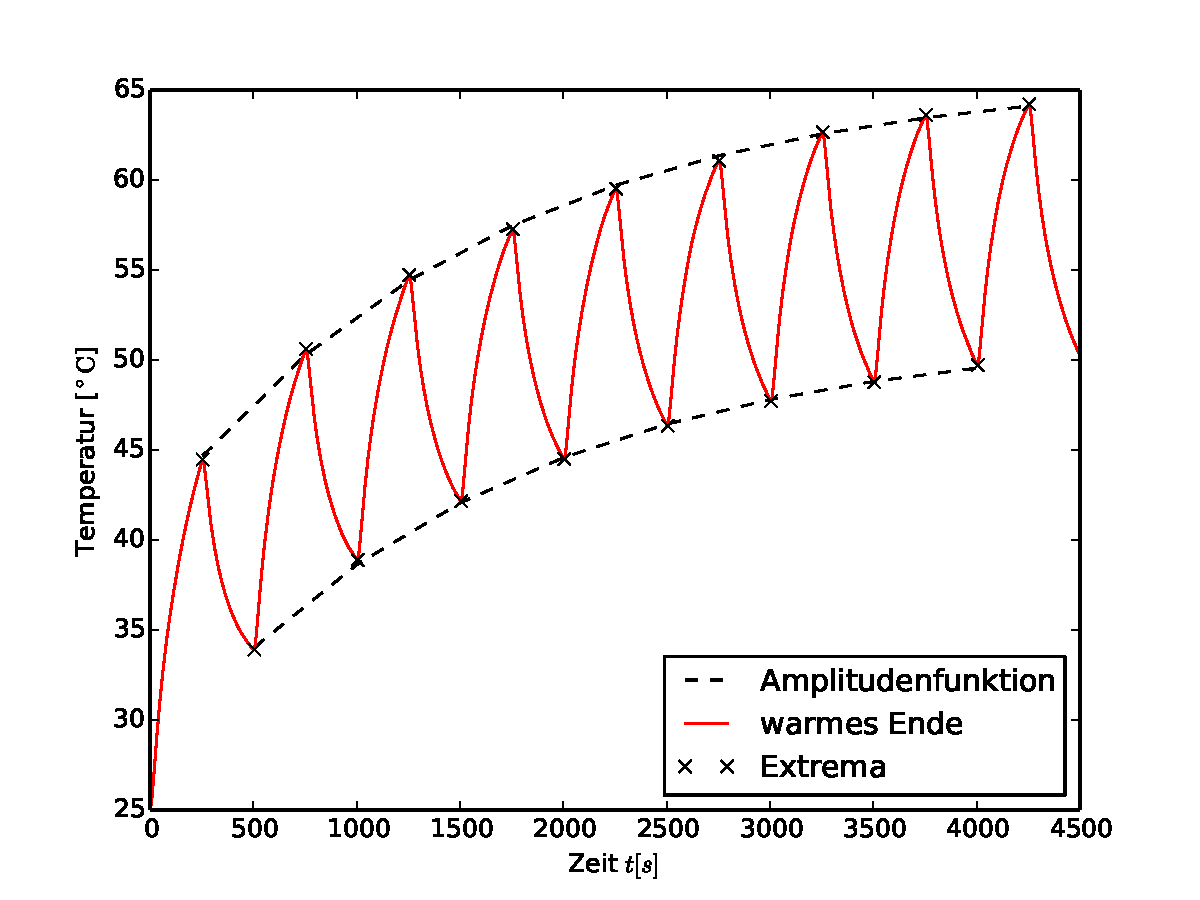
\includegraphics[width=\textwidth]{Bilder/M3_Alu_warm.pdf}
	\end{subfigure}
\caption{Periodische Messung bei Aluminium mit 200 Sekunden-Periode}
\end{figure}
\begin{figure}[htp]
	\label{fig:M3MessingNorm}
	\centering
	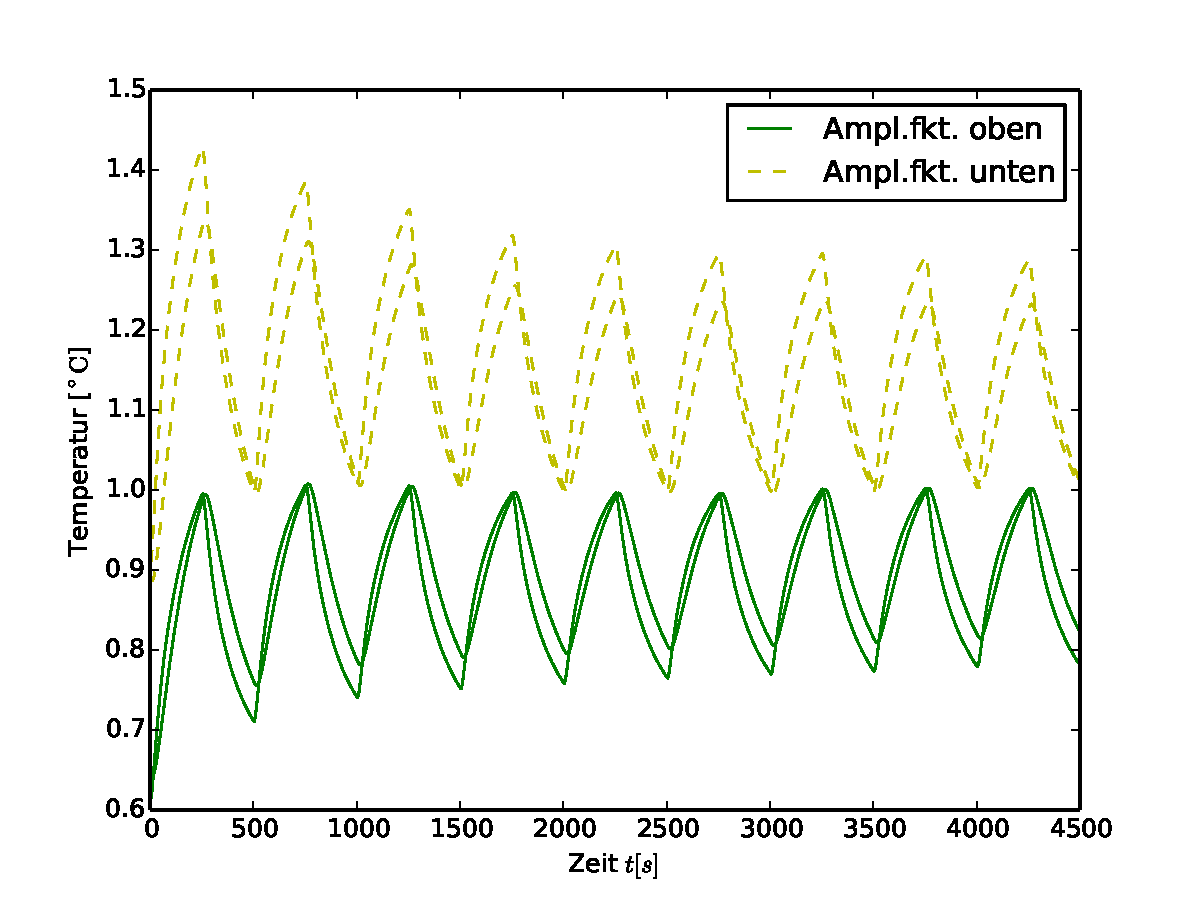
\includegraphics[width=0.8\textwidth]{Bilder/Normierungsauswahl/M3_Alu_norm.pdf}
	\caption{Normierung von Diagramm \ref{fig:M3Alu} auf Grundschwingung}
\end{figure}
\begin{figure}[htp]
	\label{fig:M3AluNorm}
	\centering
	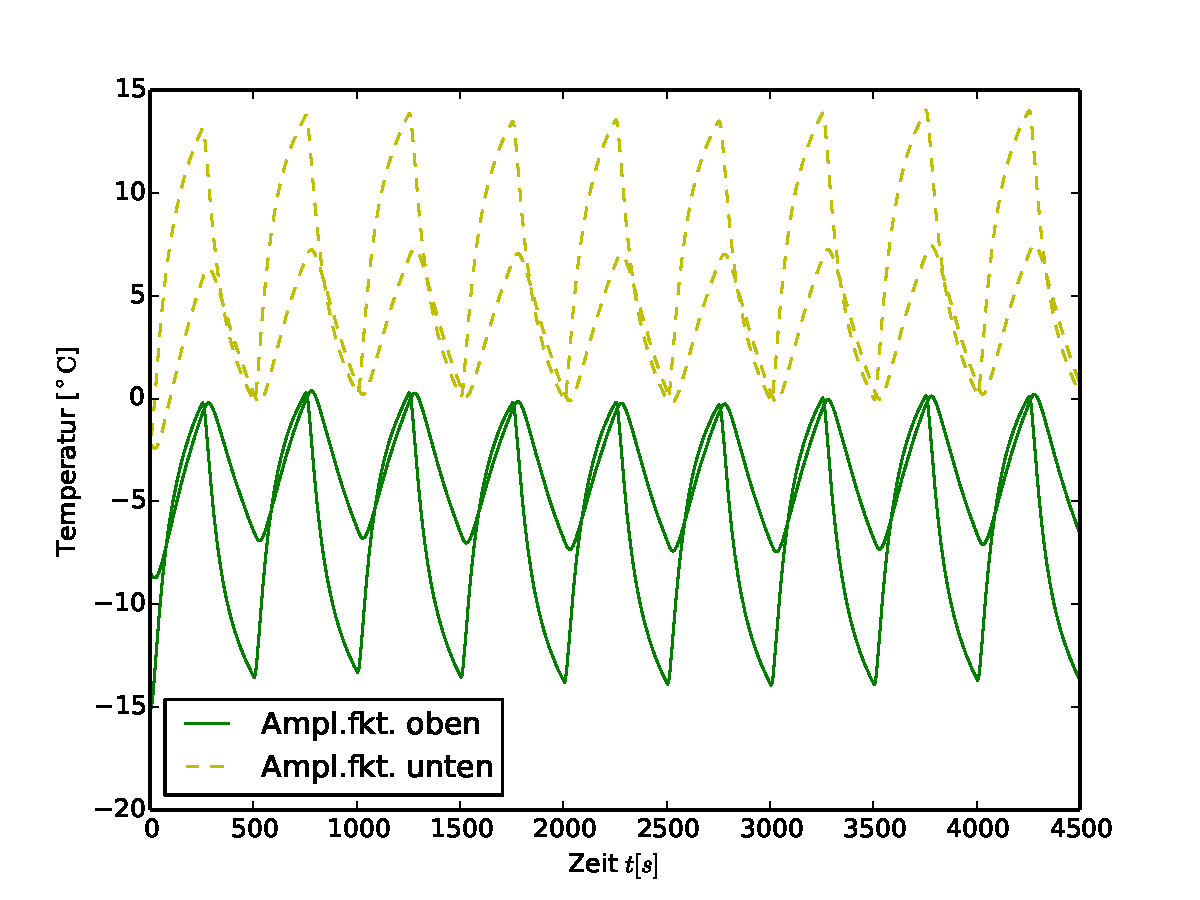
\includegraphics[width=0.8\textwidth]{Bilder/Normierungsauswahl/M3_Messing_norm.pdf}
	\caption{Normierung von Diagramm \ref{fig:M3Messing} auf Grundschwingung}
\end{figure}
\begin{figure}[p]
\label{fig:M3Edelstahl}
\centering
	\begin{subfigure}{0.9\textwidth}
	\centering
	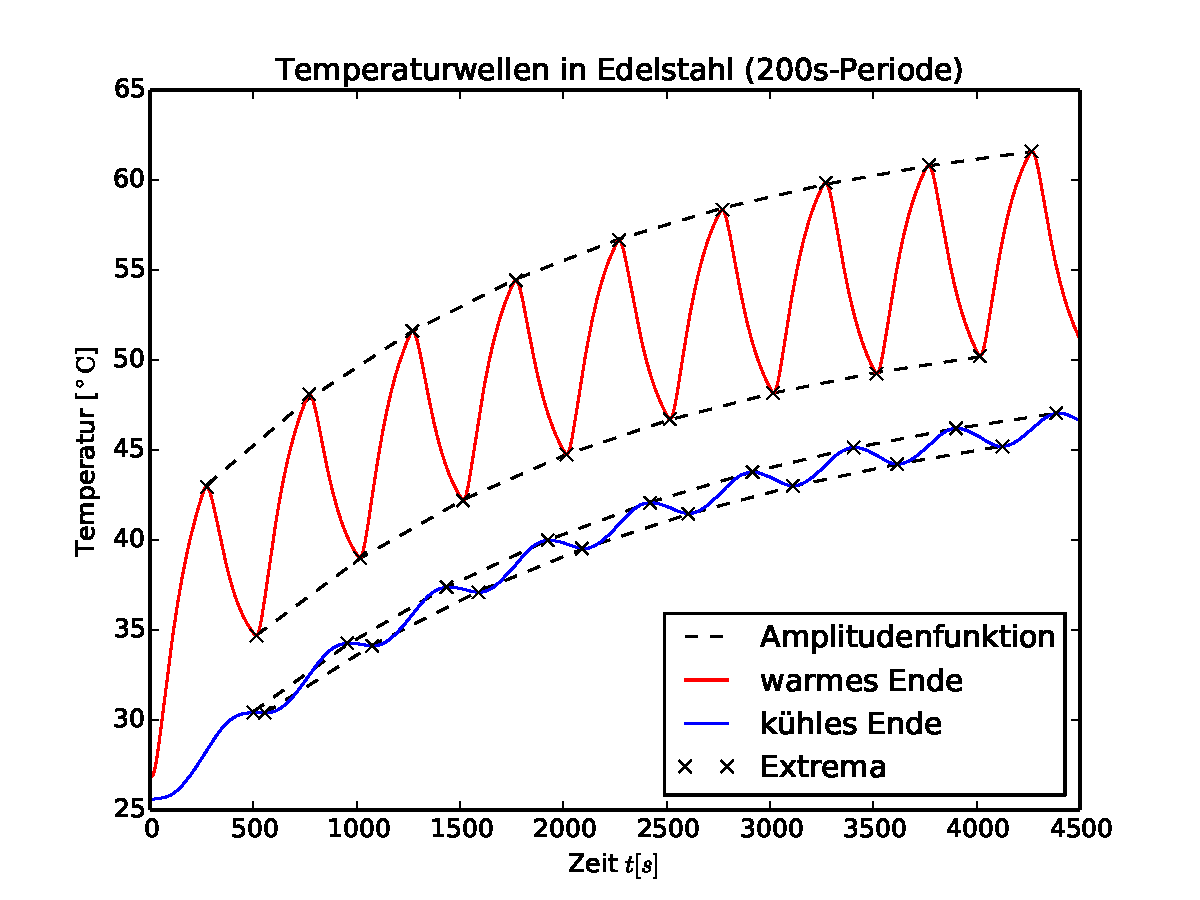
\includegraphics[width=\textwidth]{Bilder/M3_Edelstahl.pdf}
	\end{subfigure}
	\begin{subfigure}{0.9\textwidth}
	\centering
	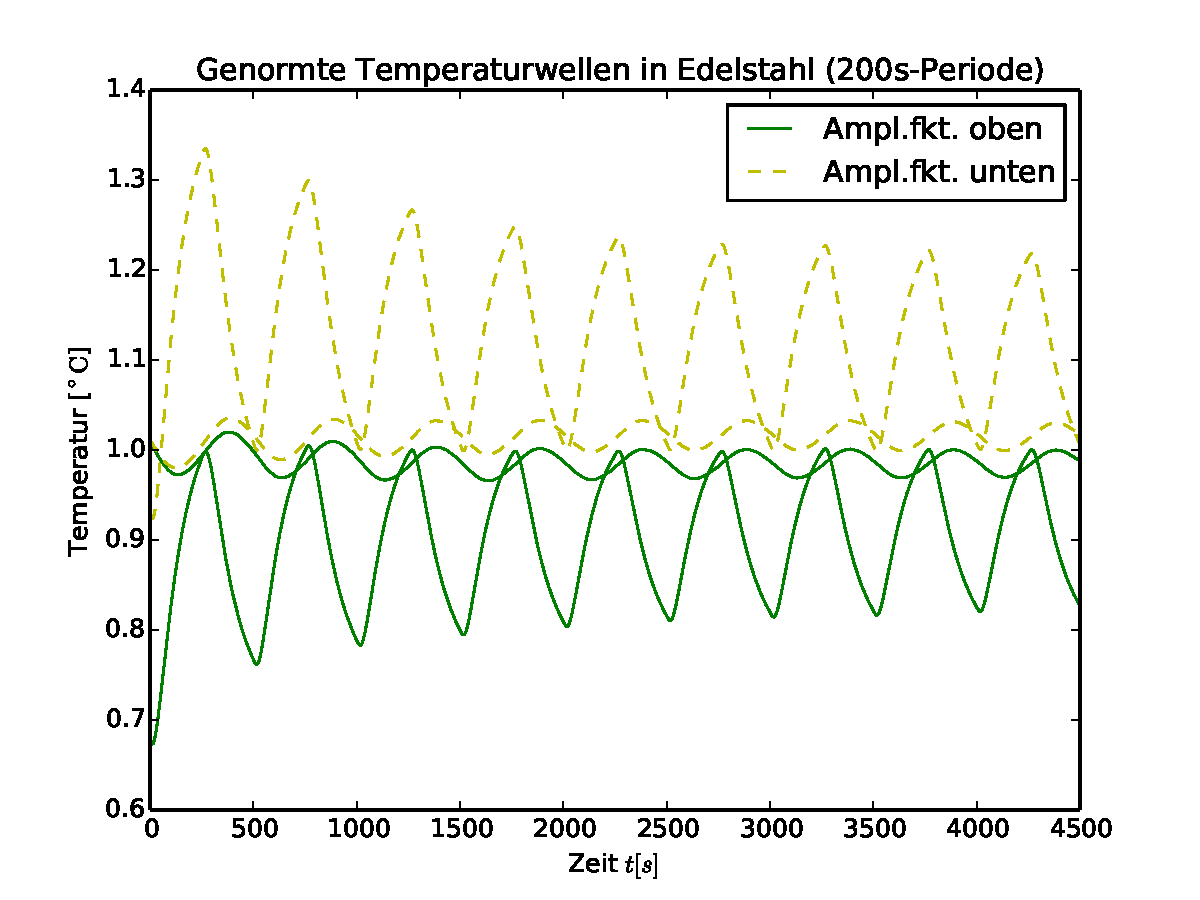
\includegraphics[width=\textwidth]{Bilder/Normierungsauswahl/M3_Edelstahl_norm.pdf}
	\end{subfigure}
\caption{Periodische Messung bei Edelstahl mit 200 Sekunden-Periode sowie Normierung auf Grundschwingung}
\end{figure}
